% !TeX spellcheck = russian-aot
\documentclass[a4paper, fontsize=14pt]{article} 

%\documentclass[russian,utf8]{eskdtext} 
\usepackage{course_work}
\addbibresource{report.bib}
\bibliography{report.bib}
%\usepackage{graphs/gnuplot-lua-tikz}
%\setcounter{page}{4} %в зависимости от того, какой по счёту страницей должно
%быть оглавление!
%\usepackage{pstricks}
\newcommand{\divop}{\operatorname{div}}
\newcommand{\gradop}{\operatorname{grad}}

\begin{document} 
	%\includepdf[pages=1-3]{cover.pdf} \newpage \tableofcontents
	%\newpage 	
	\tableofcontents
	\newpage
	\section*{Введение} 
	\addcontentsline{toc}{section}{Введение}
	\begin{comment}
	Проведение геологоразведочных мероприятий позволяет определять структуру
	и состав грунта, что, в свою очередь, позволяет обнаруживать новые
	месторождения полезных ископаемых, а также делать заключения о
	целесообразности разработки того или иного месторождения.
	Одним из наиболее используемых, эффективных и надежных методов,
	применяемых в геологоразведке, является сейсморазведка, совмещающая в себе
	относительно невысокую стоимость и высокую точность получаемых данных.

	Актуальность применения быстрых методов решения прямых и обратных механических задач обусловлена необходимостью постоянного совершенствования методов геофизического исследования и повышения эффективности разведки нефтегазовых месторождений. Сейсмическое моделирование и миграция являются неотъемлемыми компонентами процесса интерпретации сейсмических данных и предоставляют ценную информацию о структуре и свойствах залежей. В свете постоянно меняющихся условий в нефтегазовой промышленности, эти методы становятся все более важными для обеспечения точности и достоверности геологической информации.
	\end{comment}
	Определения некоторых терминов, использующихся в данной работе:
	
	Сейсмическое моделирование -- это ...
	
	Сейсмическая миграция -- это ...
	
	Функция Грина -- ...
	
%	Сейсмотрасса -- ...
	
	Целью данной работы является разработка численных алгоритмов интегральных методов решения задач сейсмического моделирования и миграции. 
	
	Для достижения поставленной цели необходимо решить следующие задачи:
	\begin{enumerate}
		\item Вывести формулу решения задачи сейсмического моделирования в интегральном виде.
		\item Вывести формулу сейсмической миграции.
		\item Выполнить программную реализацию алгоритмов интегрального метода решения задач моделирования и миграции.
		\item Провести серию вычислительных экспериментов для решения задачи на конкретном наборе данных.
	\end{enumerate}

	
	\newpage
	\section{Моделирование} 
	\subsection{Постановка задачи сейсмического моделирования} 
	\begin{figure}[h]
		
		\centering
		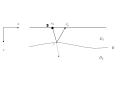
\includegraphics{migration_fig.pdf}
		
		\caption{Модель среды}
		\label{fig:mig}
	\end{figure}
	Рассмотрим задачу нахождения значения скалярного волнового поля на поверхности
	наблюдения.
	Допустим задана поверхность, ограничивающая некоторую область пространства
	$D=[0,X]\times [0,Y]\times [0,Z]$, изображённую на рисунке \ref{fig:mig}.
	Область пространства $D$ разделена на слои $D_1$ и $D_2$ границей $B$, с постоянной
	скоростью звука $c_1$ и $c_2$ соответственно.
	На границе находятся точечные источники колебаний $S$, которые возбуждают
	акустическую волну.
	
	Необходимо по данным характеристикам источников найти значение отражённого волнового поля
	на поверхности наблюдения $z=0$.
	
%	\section{Волновое уравнение}


	%%%%%%%%%%%%%%%%%%%%%%%%%%%%%%%%%%%
	\subsection{Функция Грина} 
		Решение данной задачи можно получить при помощи решения
	дифференциального волнового уравнения \ref{eq:wav}. 
	\begin{equation}
		\frac{\partial^2 P}{\partial x^2} + \frac{\partial^2 P}{\partial y^2} +
		\frac{\partial^2 P}{\partial z^2} - \frac{1}{c^2} \frac{\partial^2 P}{\partial
			t^2} = -F(x,y,z,t)   
		\label{eq:wav}	
	\end{equation}
	
	Рассмотрим мгновенный точечный источник колебаний в трёхмерном пространстве.
	Тогда правая часть уравнения \ref{eq:wav} будет иметь вид \cite{zhdanov1988}
	\begin{equation}
		F(x,y,z,t) = \delta(t-t')\delta(x-x')\delta(y-y')\delta(z-z')
		\label{eq:ptsrc}
	\end{equation}
	Где $\delta(x)$ -- это дельта-функция Дирака.
	\begin{equation}
		\delta(x)=\begin{cases}
			\infty,&x=0\\
			0,&x\neq 0
		\end{cases}
		\label{eq:deltadef}
	\end{equation}	
	Решением уравнения \ref{eq:wav} с правой частью \ref{eq:ptsrc} является функция
	Грина для волнового уравнения в трёхмерном пространстве.
	
	Пусть источник колебаний находится в начале координат и время импульса $t' = 0$. 
	
	Так как правая часть уравнения равна 0 везде, кроме точки $O(0,0,0)$, поэтому 
	$G$ удовлетворяет уравнению \ref{eq:uwav} всюду, кроме начала координат
	\begin{equation}
		\frac{\partial^2 G}{\partial x^2} + \frac{\partial^2 G}{\partial y^2} +
		\frac{\partial^2 G}{\partial z^2} - \frac{1}{c^2} \frac{\partial^2 G}{\partial
			t^2} = 0.
		\label{eq:uwav}
	\end{equation}
	Учитывая сферическую симметрию функции Грина, перейдём в уравнении \ref{eq:uwav} к сферической системе координат
	\begin{equation}
		\frac{1}{r^2}\frac{\partial}{\partial r}\left( r^2 \frac{\partial G}{\partial r} \right)- \frac{1}{c^2} \frac{\partial^2 G}{\partial
			t^2} = 0.
		\label{eq:uswav}
	\end{equation}
	Воспользовавшись равенством $\frac{1}{r}\frac{\partial}{\partial r}\left(r^2\frac{\partial G}{\partial r}\right) = \frac{\partial^2}{\partial r^2}\left(rG\right)$ преобразуем уравнение \ref{eq:uswav}:
	\begin{equation}
		\frac{\partial^2}{\partial r^2}\left( r  G\right)- \frac{1}{c^2} \frac{\partial^2 }{\partial
			t^2}\left(r G\right) = 0.
		\label{eq:uswav2}
	\end{equation}
	Таким образом мы смогли свести уравнение к одномерному волновому уравнению относительно $F(r,t) = rG$. При помощи замены переменных $\xi = t - \frac{r}{c}$, $\eta = t+\frac{r}{c}$ к простому виду:
	\begin{equation}
		\frac{\partial^2}{\partial \xi \partial \eta} F = 0	
		\label{eq:canonwav}
	\end{equation}
	Интегрируя уравнение \ref{eq:canonwav}, выразим значение функции Грина из решения дифференциального уравнения:
	\begin{equation}
		G(x,y,z,t) = \frac{1}{r}f\left(t-\frac{r}{c}\right) + \frac{1}{r} g\left(t+\frac{r}{c}\right),
		\label{eq:canonsol}
	\end{equation}
где $r = \sqrt{x^2+y^2+z^2}$.

Первое слагаемое выражения \ref{eq:canonsol} описывает сферическую волну, которая распространяется от начала координат в бесконечность, а второе слагаемое -- сферическую волну из бесконечности к началу координат. Поскольку, по условиям задачи, источником колебания является единственный источник, то функцию $g$ примем равной нулю.  Чтобы найти функцию  $f$  подставим решение \ref{eq:canonsol} в уравнение \ref{eq:wav}. 
\begin{equation}
	\Delta \left[ \frac{1}{r}f\left(t-\frac{r}{c}\right) \right] - \frac{1}{c^2} \frac{\partial^2 }{\partial
		t^2}\left[ \frac{1}{r}f\left(t-\frac{r}{c}\right) \right]  = - \delta(t)\delta(x)\delta(y)\delta(z)
		\label{eq:fwav}
\end{equation}
Используя равенство $\Delta\left(\frac{1}{r}\right) = -4\pi \delta(x)\delta(y)\delta(z)$, можно привести уравнение \ref{eq:fwav}
к виду 
\begin{equation}
	-4\pi f(t) \delta(x) \delta(y) \delta(z)  = \delta(x) \delta(y) \delta(z) \delta(t),
\label{eq:fdel}	
\end{equation}
откуда можно выразить значение функции Грина:
\begin{equation}
	G(x,y,z,t) = -\frac{1}{4\pi r} \delta \left(t - \frac{r}{c}\right),
\label{eq:green3d0}	
\end{equation}  
где $r = \sqrt{x^2+y^2+z^2}$.

При выводе формулы \ref{eq:green3d0} использовалось предположение,  что источник находится в начале координат  и посылает импульс в момент времени $t' = 0$. При переходе к произвольному положению источника 
формула для функции Грина имеет вид
\begin{equation}
	G(\bar{r}',t'|\bar{r},t)= \frac{1}{4\pi|\bar{r}'-\bar{r}|}
	\delta\left(t'-t-\frac{|\bar{r}'-\bar{r}|}{c}\right)
\label{eq:green3d}
\end{equation}

	Такая функция Грина называется запаздывающей функцией Грина, так как эффект,
	наблюдаемый в точке $\bar{r}'$ в более поздний момент времени $t'$ вызывается
	возмущением,
	которое произошло в точке $\bar{r}$ в более ранний момент времени $t$.

	
	Для волнового уравнения с произвольной правой частью $F(x,y,z,t)$ можно
	записать формулу представления решения 
	в аналитическом виде при помощи функции Грина, введя вектор $\bar{r} = (x,y,z)$: \cite{zhdanov2007}
	\begin{equation}
		P(\bar{r}',t')=\iiint\limits_{D_1} \int\limits_{-\infty}^{+\infty}
		F(\bar{r},t) G(\bar{r}',t'|\bar{r},t)\,dt\,dv
	\end{equation}
	%TODO ссылка на литру
	
% DONE Связь излучаемого и отраженного волнового поля через коэффициент отражения

% Кирхгоф пока что не нужен
% да блин не нужен тут Борн. Тут сослаться надо на книжку и  сказать, что \lambda = (с1-с2)/(c1+c2)

	
	\subsection{Формула Кирхгофа}
	Для вычисления значения отражённого волнового поля на поверхности наблюдения необходимо 
	рассмотреть как связано значение поля на отражающей границе и значения поля в других точках области, которую ограничивает эта поверхность.   
	% DONE ссылку на будущее уравнение убрать
	Рассмотрим  некоторую ограниченную область пространства $D$, в пределах которой задано скалярное волновое поле, удовлетворяющее следующему уравнению:
	
	\begin{equation}
		\diff[2]{P}{x}  + \diff[2]{P}{y} +
		\diff[2]{P}{z}  - \frac{1}{c^2} \frac{\partial^2 P}{\partial
			t^2} = 0.
		\label{eq:uwav2}
	\end{equation}
	
	 Положим, что граница $S$ области $D$ является кусочно-гладкой. Так как область $D$ ограничена и имеет кусочно-гладкую границу, тогда по
	теореме Остроградского-Гаусса справедливо соотношение
	\begin{equation}
		\iiint\limits_D \divop F \, dv = \iint\limits_S F \cdot n \, ds 
		\label{eq:vgauss}
	\end{equation}
	Для любых гладких функций $u$ и $v$ справедливо соотношение 
	\begin{equation}
		\divop (u \gradop v) = u\Delta v + \gradop u \cdot \gradop v.
		\label{eq:divgrad1}
	\end{equation}
	Симметрично можно записать:
	\begin{equation}
		\divop (v \gradop u) = v\Delta u + \gradop v \cdot \gradop u.
		\label{eq:divgrad2}
	\end{equation}
	Путём вычитания из уравнения \ref{eq:divgrad1} уравнения \ref{eq:divgrad2} получим 
	\begin{equation}
		\divop (u \gradop v - v \gradop u)  = u\Delta v - v \Delta u
		\label{eq:divgraddiff}
	\end{equation}
	Пусть векторы $r = (x,y,z) \in S$ и $r' = (x',y',z') \in D$ -- это радиус-векторы точек на поверхности $S$ и области $D$ соответственно.
	Положим 
	\begin{eqnarray}
		u(x,y,z,t) =& P(x,y,z,t),\label{eq:subsu}\\
		v(x,y,z,t) = &G(x',y',z',t'|x,y,z,t),\label{eq:subsv}
	\end{eqnarray}	
	тогда 
	% DONE  Ввести вектора r и r'
	% DONE ввести обозначения для случаев, где функция без аргументов
\begin{eqnarray}
	\Delta u =& \frac{1}{c^2} \diff[]{P}{t},\label{eq:subsdu}\\
	\Delta v = &\delta (r' - r) \delta(t' - t) + \frac{1}{c^2} \diff [2]{G(r' -r,t'-t)}{t},\label{eq:subsdv}
\end{eqnarray}
где $r=(x,y,z)$. Для краткости обозначим
	\begin{align*}
		P =& P(r,t) \\
		G =& G(r',t'|r,t)
	\end{align*}
	Проинтегрируем уравнение \ref{eq:divgraddiff} по времени
	\begin{equation}
		\divop \int\limits_{-\infty}^{+\infty} [P \gradop G - G \gradop P ]\, dt=  P\delta(r-r') +\frac{1}{c^2}\int\limits_{-\infty}^{+\infty}\left[P\diff[2]{G}{t} - G \diff[2]{P}{t}\right]\,dt.
		\label{eq:ugauss}
	\end{equation}
	Интегрированием по частям можно показать, что 
	$$
	\int\limits_{-\infty}^{+\infty}\left[P\diff[2]{G}{t} - G \diff[2]{P}{t}\right]\,dt = 0.
	$$
	Введём обозначение 
	$$
		F(x,y,z,t') = \int\limits_{-\infty}^{+\infty} [P \gradop G - G \gradop P ]\, dt
	$$
	Тогда из уравнений \ref{eq:ugauss} и \ref{eq:vgauss} следует
	\begin{equation}
		\iiint\limits_D P\delta(r-r') \, dv = \iint\limits_S F \cdot n \, ds 
	\end{equation}
Таким образом, 
	% TODO не физично
	% TODO подставить все до конца раздела
	\begin{equation}
		P(r',t') = \iint\limits_{\partial D} \int\limits_{-\infty}^{+\infty} 
	[G(r',t'|r,t)\partial_n P(r,t) 
	- P(r,t)\partial_n G(r',t'|r,t)] \,dt\,ds
	\label{eq:kir}
	\end{equation}
	
	
	Это соотношение носит название интегральной формулы Кирхгофа.
	Интегральная
	формула Кирхгофа показывает, как можно восстановить волновое поле внутри области,
	ограниченной некоторой поверхностью, по значениям этого поля (и его нормальной
	производной) на границе области.
	
	Для ...%TODO написать про формулу из Покровской

	\subsection{Уравнение Гельмгольца}
	Для дальнейших рассуждений будет удобно перейти от временной области в частотную. Представим поле $P(r,t)$ как суперпозицию полей в частотной области $p(r,\omega)$:
	\begin{equation}
		P(r,t) =  \int_{-\infty}^{\infty} p(r,\omega) e^{i\omega t}\, d\omega
	\end{equation}
	Применим преобразование Фурье к волновому уравнению \ref{eq:wav}:
	\begin{equation}
		\int_{-\infty}^{\infty} \left[ \nabla^2 P(r,t) + \frac{1}{c^2}\diff[2]{P(r,t)}{t}\right] e^{-i\omega t} \, dt = - \int_{-\infty}^{\infty}   F(r,t) e^{-i\omega t} \, dt
	\end{equation}
	По свойствам преобразования Фурье производная по времени переходит в частотной области в умножение на коэффициент 
	$i\omega$. В результате получаем уравнение, называемое {\it уравнением Гельмгольца}:
	\begin{equation}
		\nabla^2 p(r,\omega) + \frac{\omega^2}{c^2}p(r,\omega) = - f(r,\omega)
		\label{eq:helmholtz}
	\end{equation}
	\subsection{Коэффициент отражения}
	% Из Гельмгольца вывести
	% TODO взять условия равенства  давлений на границе раздела сред
	Запишем уравнение из 	
	% разделение поля на фоновое и аномальное.
	
	
	При отражении отражении акустической волны от границы на поверхности раздела должны быть равны давления и нормальные скорости в обеих средах.

	
	Используя известную  зависимость между звуковым давлением $p$ и нормальной скоростью $\diff{p}{n}$, запишем выражения звуковых давлений через волновое сопротивление, соответственно, в падающей ($p_0$), отражённой ($p_1$) и прошедшей ($p_2$) волнах. \cite{brehovskih} 
	% TODO ссылку на нормальную литературу.
	
	
	%\begin{comment}
	\begin{eqnarray}
		P_0 = v_0 \rho_1 c_1 \label{eq:pvrc0} \\
		P_1 = - v_1 \rho_1 c_1 \label{eq:pvrc1}\\
		P_2 = v_2 \rho_2 c_2 \label{eq:pvrc2}
	\end{eqnarray}
	Условия неразрывности звукового давления и колебательной скорости на границе сред:
	\begin{eqnarray}
		P_0 + P_1 = P_2 \label{eq:p012}\\
		v_0 + v_1 = v_2 \label{eq:v012}
	\end{eqnarray}
	Выражая из уравнений \ref{eq:pvrc0}, \ref{eq:pvrc1} и \ref{eq:pvrc2} значения колебательной скорости и подставляя их в выражение \ref{eq:v012}, получим систему линейных уравнений относительно значений звукового давления:
	\begin{eqnarray}
		P_0 + P_1 =& P_2 \nonumber\\
		\frac{P_0}{\rho_1 c_1} - \frac{P_1}{\rho_1 c_1} =& \frac{P_2}{\rho_2 c_2} 
	\end{eqnarray}
	Из решения данной линейной системы можно выразить отношение $\Lambda$ между давлениями падающего и отражённого полей:
	\begin{equation}
		P_1 = P_0 \cdot \frac{\rho_2 c_2 - \rho_1 c_1}{\rho_1 c_1 + \rho_2 c_2 }.
		\label{eq:nreflratio}
	\end{equation}
	
	Введём обозначения для коэффициентов отражения и прохождения:
	\begin{gather}
		\beta =  \frac{\rho_2 c_2 - \rho_1 c_1}{\rho_1 c_1 + \rho_2 c_2 },\\
		\alpha =  \frac{\rho_1 c_1}{\rho_1 c_1 + \rho_2 c_2 }.
	\end{gather} 
	%\end{comment}
	Это соотношение описывает отражённое волновое поле соответствующее  волне, падающей перпендикулярно границе раздела двух сред. 
	Если рассматривать падение звука под некоторым углом, то ширины падающего, отражённого и преломлённого лучей будут  пропорциональны косинусам соответствующих углов.\cite{zakharov} 
	В таком случае уравнение закона сохранения кинетической энергии при падении волны под углом $\theta_1$ и преломлении под углом $\theta_2$ к нормали границы сред примет вид:
	\begin{equation}
		\frac{\rho_1 \lambda_1 v^2 \cos \theta_1}{2} = \frac{\rho_1 \lambda_1 (v\beta)^2 \cos \theta_1}{2} + \frac{\rho_2 \lambda_2 \cos \theta_2 (v\alpha)^2 }{2}
		\label{eq:reflecl}
	\end{equation}
	Векторное уравнение сохранения количества движения содержит в знаменателях каждого члена косинусы направления колебаний продольных волн в каждом луче:
	\begin{equation}
		\rho_1 \lambda_1 \cos \theta_1 \cdot \frac{v}{\cos \theta_1} = \frac{\rho_1 \lambda_1 \cos \theta_1 \cdot v \beta}{\cos \theta_1} + \frac{\rho_2 \lambda_2 \cos \theta_2 \cdot v\alpha}{\cos\theta_2}
		\label{eq:reflicl}
	\end{equation}
	Из решения системы уравнений \ref{eq:reflecl} и \ref{eq:reflicl} аналогично можно выразить коэффициенты отражения и прохождения:
	\begin{gather}
		\beta =  \frac{\rho_2 c_2 - \rho_1 c_1}{\rho_1 c_1 + \rho_2 c_2 },\\
		\alpha =  \frac{\rho_1 c_1}{\rho_1 c_1 + \rho_2 c_2 }.
	\end{gather} 
	
	Рассмотрим область пространства $D_1$, ограниченную снизу отражающей поверхностью $B$. 
	Так как волновое поле, созданное источником, испытывает отражение на границе, то отражённое поле можно приблизительно описать при помощи коэффициента отражения\cite{zhdanov2007}
	\begin{eqnarray}
		P_1(r,t') = \Lambda(r) P_0(r,t'), \label{eq:lambda}\\
		\diff{P_1(r,t') }{n} = - \Lambda(r) \diff{P_0(r,t')}{n}. \label{eq:lambdadnp0}
	\end{eqnarray}
	При этом коэффициент отражения на границе двух однородных областей можно вычислить как
	\begin{equation}
		\Lambda = \frac{\rho_2 c_2-\rho_1 c_1}{\rho_1 c_2+\rho_1 c_1}
		\label{eq:refl}
	\end{equation}

	%DONE страница 536 (djvu 273) Теория обратных задач
	% коэффициент отражения 567
	\subsection{Приближение Кирхгофа}
	Рассмотрим волновое поле в частотной области.Оно удовлетворяет уравнению Гельмгольца с различными правыми частями выше и ниже отражающей поверхности $B$ \cite{zhdanov2007}:
	\begin{equation}
		\nabla^2 p(r,\omega) + \frac{\omega^2}{c^2(r)}p(r,\omega) = \begin{cases}
			-f(r,\omega), & r \in D_1 \\
			0,            & r \in D_2
		\end{cases}
		\label{eq:helmp}
	\end{equation} 
	Можно представить суммарное поле как суперпозицию первичного и отражённого полей над отражающей поверхностью $B$, и как преломлённую волну $p^T(r,\omega)$ ниже отражателя:
	\begin{equation}
		p(r,\omega) = \begin{cases}
			p^i(r,\omega)+p^s(r,\omega),& r \in D_1 \\
			p^T(r,\omega), & r \in D_2
		\end{cases}
	\end{equation}
	Слагаемые удовлетворяют следующим уравнениям:
	\begin{eqnarray}
		\nabla^2 p^i(r,\omega) + \frac{\omega^2}{c^2(r)}p^i(r,\omega) =-f(r,\omega), r \in D_1,\\
		\nabla^2 p^s(r,\omega) + \frac{\omega^2}{c^2(r)}p^s(r,\omega) = 0, r \in D_1,\\
		\nabla^2 p^T(r,\omega) + \frac{\omega^2}{c^2(r)}p^T(r,\omega) =0, r \in D_2
	\end{eqnarray}
	%TODO написать про условия Зоммерфельда : зачем они нужны
	Также предположим, что все волновые поля удовлетворяют условиям излучения Зоммерфельда:
	\begin{eqnarray}
		rp(r,\omega) = C < \infty\\
		\lim\limits_{r\to\infty} |r|\left[\diff{p(r,\omega)}{r} - i\frac{\omega}{c}p(r,\omega)\right] =0
	\end{eqnarray}
	Воспользуемся формулой Кирхгофа для выражения волнового поле в точке $r'\in D_1$.
	\begin{equation}
		p^s(r',\omega)= \iint\limits_B \left[ p^s(r_b,\omega)\diff{ G(r'|r_B;\omega)}{n}- G(r'|r_B;\omega)\diff{p^s(r_b,\omega)}{n}\right] \,ds_B
	\end{equation}
	Учитывая приближения для отражённой волны \ref{eq:lambda} и \ref{eq:lambdadnp0}, можно получить формулу для продолжения отражённого волнового поля в частотной области:
	\begin{equation}
		p^s(r',\omega)= \iint\limits_B \Lambda(r_B) \diff{[p^i(r_B,\omega)\cdot G(r'|r_B,\omega)]}{n} \,ds_B.
		\label{eq:kirapxfrq}
	\end{equation}
	Применим обратное преобразования Фурье к уравнению \ref{eq:kirapxfrq}, чтобы перейти от частотной области к временной.
	\begin{equation}
			P^s(r',t')= \iint\limits_B \Lambda(r_B) \diff{}{n} \left[\int\limits_{-\infty}^{+\infty}P^i(r_B,t)G(r',t'|r_B,t)\,dt\right]\,ds_B.
			\label{eq:kirapxt}
	\end{equation} 
	Теперь можно подставить аналитическое выражение функции Грина \ref{eq:green3d} в формулу \ref{eq:kirapxt}.\cite{fomel}
	%TODO где свертка?
	\begin{equation}
		P^s(r',t')= \iint\limits_B \Lambda(r_B) \diff{}{n} \left[\frac{f\left(t - \frac{|\bar{r}_B-\bar{r}_s|}{c_1} -\frac{|\bar{r}'-\bar{r}_B|}{c_1} \right)}{16\pi^2|\bar{r}_B-\bar{r}_s|\cdot |\bar{r}'-\bar{r}_B|}\right]\,ds_B.
		\label{eq:kirapxgt}
	\end{equation} 
	%\begin{comment}
	\subsection{Приближение Борна}
	Представим скорость распространения волны в виде
	\begin{equation}
		\frac{1}{c^2(r)} = \frac{1+a(r)}{c_1^2}.
	\end{equation}
	Обозначим значение, обратное по величине скорости волны, как медленность 
	\begin{gather*}
		s = \frac{1}{c} \\
		s_1 = \frac{1}{c_1} \\
		s_2 = \frac{1}{c_2}
	\end{gather*}
	Таким образом функция $a(r)$ является квадратом нормированной аномальной медленности:
	$$
		a(r) = \frac{s^2 - s_1^2}{s_1^2} = \frac{\Delta s^2}{s_1^2}
	$$
	Падающее волновое поле удовлетворяет волновому уравнению в области $D_1$:
	\begin{equation}
		\nabla^2 P_0 - \frac{1}{c_1^2}\diff[2]{P_0}{t} = 0.
		\label{eq:wavp0}
	\end{equation}
	Преломлённое волновое поле также является решением волнового уравнения, но в области $D_2$ с другой скоростью звука:
	\begin{equation}
		\nabla^2 P_2 - \frac{1}{c_2^2}\diff[2]{P_2}{t} = 0.
		\label{eq:wavp2}
	\end{equation}
	Из условия \ref{eq:p012} непрерывности значения  волнового поля на границе однородной области можно переписать уравнение \ref{eq:wavp2} в виде
	\begin{equation}
		\nabla^2 P_0 + \nabla^2 P_1 - \frac{1}{c_2^2}\diff[2]{P_0}{t} - \frac{1}{c_2^2}\diff[2]{P_1}{t}  = 0.
		\label{eq:wavp01sum}
	\end{equation}
	Подставим в выражение $\nabla^2 P_0$ из уравнения \ref{eq:wavp0}, и
	тогда отражённое волновое поле будет удовлетворять уравнению \cite{bleistein2012mathematical}
	\begin{equation}
		 \nabla^2 P_1 - \frac{1}{c_2^2}\diff[2]{P_1}{t}  = - \frac{1}{c_1^2}\diff[2]{P_0}{t} + \frac{1}{c_2^2}\diff[2]{P_0}{t}.
	\end{equation}
	Так как отражённая волна распространяется в области $D_1$, то она удовлетворяет следующему неоднородному волновому уравнению:
	\begin{equation}
		\nabla^2 P_1 - \frac{1}{c_1^2}\diff[2]{P_1}{t}  = \left(\frac{1}{c_2^2} - \frac{1}{c_1^2}\right)\left(\diff[2]{P_0}{t} + \diff[2]{P_1}{t}\right).
		\label{eq:wavp1inh}
	\end{equation}
	Используя введённые ранее обозначения, перепишем уравнение \ref{eq:wavp1inh} следующим образом:
	\begin{equation}
		\nabla^2 P_1 - \frac{1}{c_1^2}\diff[2]{P_1}{t}  = \Delta s^2 \cdot \diff[2]{P_2}{t}.
	\end{equation}
	Следовательно, решение этого неоднородного дифференциального уравнения можно выразить через функцию Грина:
	\begin{equation}
		P_1(r',t')   = \iiint\limits_{D_1} \int\limits_{-\infty}^{\infty} \Delta s^2 \cdot \left(\diff[2]{P_0(r,t)}{t}+\diff[2]{P_1(r,t)}{t}\right) G(r',t'|r,t)\, dt \, dv.
	\end{equation}
	Приближение Борновского типа состоит в том, чтобы положить отражённое поле под знаком интеграла равным нулю:
	\begin{equation}
		P_1(r',t')   = \iiint\limits_{D_1} \int\limits_{-\infty}^{\infty} \Delta s^2 \cdot 	\diff[2]{P_0(r,t)}{t} G(r',t'|r,t)\, dt \, dv.
	\end{equation}
	%\end{comment}
	%DONE: !!! Оттражение от наклонной плоскости!!
	\begin{comment}
	\subsection{Отражение от наклонной плоской границы}
		Если подставить в выражение \ref{eq:kir} функцию Грина \ref{eq:green3d} в явном виде и проинтегрировать по времени, то получится \cite{magisters}
	\begin{align}
		P(r',t') =& \frac{1}{4\pi} \iint_B	\left[ \frac{1}{c|r'-r|}\partial_n|r'-r|\frac{\partial \tilde{P}(r,t')}{\partial t'} \right.\nonumber \\
		&\left. - \partial_n
		\left(\frac{1}{|r'-r|}\right)\tilde{P}(r,t') +\frac{1}{|r'-r|}\partial_n \tilde{P}(r,t')\right]\,ds
		\label{eq:kirgreen3d}
	\end{align}
	где $\tilde{P}(r,t) = P\left(r,t - \frac{|r'-r|}{c}\right)$ -- волна запаздывания.
	
		Пусть поверхность $B$ является плоскостью, заданной уравнением 
		$$
			Ax+By+Cz=D,
		$$ внешняя нормаль которой направлена вдоль вектора $n =(A,B,C)$, то есть $\partial_n = n \cdot \nabla$. Тогда можно аналитически вычислить значение нормальных производных
		\begin{eqnarray}
			\partial_n|r'-r| =&\frac{A(x' - x)}{|n|\cdot|r' - r|}+\frac{B(y' - y)}{|n|\cdot |r' - r|} + \frac{C(z' - z)}{|n|\cdot|r' - r|}, \\ 
			\partial_n\left(\frac{1}{|r'-r|}\right) =&  - \frac{A(x' - x)}{|n|\cdot|r' - r|^3}-\frac{B(y' - y)}{|n|\cdot |r' - r|^3} - \frac{C(z' - z)}{|n|\cdot|r' - r|^3}.
		\end{eqnarray} 
		Значения нормальной и временной производных от волны запаздывания можно вычислить численно, заменив производную на её разностный аналог, либо аналитически, если функция волны запаздывания также задана аналитически.
		
		Например, пусть волна на отражающей поверхности задана функцией
		\begin{equation}
			P(r,t) = \left( 1-2\,{\pi}^{2}{t}^{2} \right) {{\rm e}^{-{\pi}^{2}{t}^{2}}},
		\end{equation}
		тогда волна запаздывания будет иметь вид
		\begin{equation}
			\tilde{P}(r,t) = \left( 1-2\,{\pi}^{2} \left( t-{\frac {\sqrt {{x}^{2}+{y}^{2}+{z}^{2}
				}}{c}} \right) ^{2} \right) {{\rm e}^{-{\pi}^{2} \left( t-{\frac {
							\sqrt {{x}^{2}+{y}^{2}+{z}^{2}}}{c}} \right) ^{2}}}.
			\label{eq:latewavrick}
		\end{equation}
		Для удобства, обозначим $|r| = \sqrt{x^2+y^2+z^2}$. Производная по времени выражается как
		\begin{align}
\diff{\tilde{P}(r,t)}{t}=&-4\,{\pi}^{2} \left( t-{\frac { \left| r \right| }{c}} \right) {
	{\rm e}^{-{\pi}^{2} \left( t-{\frac { \left| r \right| }{c}} \right) ^
		{2}}}\nonumber\\
	&-2\, \left( 1-2\,{\pi}^{2} \left( t-{\frac { \left| r \right| }{c
}} \right) ^{2} \right) {\pi}^{2} \left( t-{\frac { \left| r \right| 
	}{c}} \right) {{\rm e}^{-{\pi}^{2} \left( t-{\frac { \left| r \right| 
			}{c}} \right) ^{2}}},
	\end{align}
	а производную по пространственной переменной $x$ можно вычислить следующим образом:
	\begin{align}
		\diff{\tilde{P}(r,t)}{x} = -4\,{\frac { \left( -2\, \left| r \right| {\pi}^{2}ct+ \left( {c}^{2}{
					t}^{2}+|r|^2 \right) {\pi}^{2}-3/2\,{c}^{2} \right) 
				\left( tc- \left| r \right|  \right) x{\pi}^{2}}{|r|{c}^{4}}{{\rm e}^{-{\frac {{\pi}^{2} \left( -tc+ \left| r
							\right|  \right) ^{2}}{{c}^{2}}}}}}.
	\label{eq:latewavrickdx}
	\end{align}
	
	Так как функция \ref{eq:latewavrick} симметрична относительно пространственных переменных, то частные производные $\diff{\tilde{P}(r,t)}{y}$ и $\diff{\tilde{P}(r,t)}{z}$
	будут иметь вид, аналогичный выражению \ref{eq:latewavrickdx}.  
	Значение производной вдоль внешней нормали плоскости $B$ можно вычислить как 
	\begin{equation}
		\diff{\tilde{P}(r,t)}{n} = \frac{A}{|n|} \diff{\tilde{P}(r,t)}{x} +
		  \frac{B}{|n|} \diff{\tilde{P}(r,t)}{y} +
		   \frac{C}{|n|} \diff{\tilde{P}(r,t)}{z},
	\end{equation}
	где $|n| = \sqrt{A^2+B^2+C^2}$.
		%Подставим значения производных в выражение \ref{eq:kirgreen3d}
		%\begin{equation}
		%	P(r',t') = \frac{1}{4\pi} \iint\limits_B
		%	\left[\frac{z'-z}{|r'-r|^2}\left(\frac{1}{c}\frac{\partial\tilde{P}(r',t')}{\partial t'}+\frac{\tilde{P}(r',t')}{|r'-r|}\right) - \frac{1}{|r'-r|}\frac{\partial\tilde{P}(r',t')}{\partial z}\right]\,ds
		%\end{equation}

\end{comment}
	

	\section{Миграция}
	\subsection{Постановка задачи сейсмической миграции}
	%FIXME: постановка задачи
	
	Пусть возбуждение и регистрация колебаний происходит на плоской горизонтальной поверхности. Пусть
	существует некоторая неизвестная граница, которую мы хотим определить, при этом распределение скорости в пространстве
	между свободной поверхностью и границей считается известным. 
	
	Такую задачу можно свести к задаче нахождения обращенного продолжения $W(r',t')$ ($t' = T-t$) поля $P(r,t)$ ($r=(x,y,0),t\in[0,T]$), зарегистрированного на поверхности $z=0$ \cite{petrashen}. 
	Под обращенным продолжением понимается решение уравнения
	\begin{equation}
		\Delta W + \frac{1}{c^2} \diff[2]{W}{t} = 0
	\end{equation}
	в области $z<0$ с нулевыми начальными условиями и граничным условием
	\begin{gather*}
		\left.W\right|_{t'=0} = 0, \\
		\left.\diff{W}{t'}\right|_{t'=0} = 0, \\
		 \left.W\right|_{z=0} = P(r,t).
	\end{gather*}
	
	Рассмотрим гипотетическую волну, двигающуюся вверх к поверхности наблюдения с направлением, которое в определённый момент времени (например, при $t = 0$) совпадает с одной из отражающих границ. Далее, очевидно, что волна будет распространяться вдоль тех же лучей, что и реальное отражённое поле <<нулевого удаления>>, которое было зарегистрировано совмещёнными источниками и приёмниками, для времени $t>0$. Это связано с тем, что лучи первичной и отражённой волн должны совпадать, если положения источников и приёмников совпадают. Это возможно только в том случае, если соответствующая траектория луча нормальна к отражающей границе. Таким образом, как и предполагаемая волна, которую мы называем восходящей волной Клербо, и реальное отражённое волновое поле, зарегистрированное совмещёнными источниками и приёмниками, они должны распространяться вдоль одних и тех же лучевых путей. Тем не менее, волне Клербо потребуется пятьдесят минут, чтобы достичь определённой точки на поверхности наблюдения, куда придёт реальная отражённая волна, которая должна пройти это расстояние дважды. Тем не менее, обе волны достигнут любой точки поверхности наблюдения одновременно, если предположить, что скорость волны Клербо в среде в два раза меньше, чем скорость реальной волны. \cite{zhdanov2007}

	\subsection{Интеграл Рэлея}
	Для восстановления волн, которые распространяются по направлению к поверхности наблюдения, в качестве фундаментального решения нужно использовать функцию, сопряжённую к функции Грина волнового уравнения.
	\begin{equation}
	\widetilde{G}( r,t|r',t')=G(r,-t|r,-t).
	\end{equation}
	В случае постоянной скорости звука, эта функция имеет вид:
	\begin{equation}
	\widetilde{G}(r,t\mid r',t')=\frac{1}{4\pi\left|r-r'\right|}\delta\left(\frac{\left|r-r'\right|}{c}+(t-t')\right).
	\end{equation}
	Для того, чтобы функция соответствовала значениям волнового поля на поверхности наблюдения, необходимо и достаточно, чтобы выполнялось равенство
	\begin{equation}
	\iint_{S}\int_{-\infty}^{\infty}{\widetilde{G}}\left(r'',t^{\prime}|r,t\right){\frac{\partial}{\partial n}}P(r,t)d t\,d s = \iint_{S}\int_{-\infty}^{\infty}P(r,t){\frac{\partial}{\partial n}}{\widetilde{G}}\left(r'',t^{\prime}|r,t\right)\,d t\,d s.
	\end{equation}
	Пусть точки $r'$ и $r''$ расположены симметрично относительно $S$. Тогда справедливы для любой точки $r\in S$
	\begin{eqnarray}
		\widetilde{{{G}}}\left({r}^{\prime\prime},t^{\prime}|{r},t\right)~~=~~\widetilde{G}\left({r}^{\prime},t^{\prime}|{r},t\right), \\
		\frac{\partial}{\partial n}\widetilde G\left({ r}^{\prime\prime},t^{\prime}|{ r},t\right)~=~-\frac{\partial}{\partial n}\widetilde G\left({ r}^{\prime},t^{\prime}|{ r},t\right).
	\end{eqnarray}
	В результате получается тождество для любого ${ r}^{\prime}\in V$.
	\begin{equation}
	\iint_{S}\int_{-\infty}^{\infty}\widetilde{G}\left({r}^{\prime},t^{\prime}|{r},t\right)\frac{\partial}{\partial n}P({r},t)d t\,d s = -\iint_{S}\int_{-\infty}^{\infty}P({ r},t){\frac{\partial}{\partial n}}\widetilde{G}\left({ r}^{\prime},t^{\prime}|{ r},t\right)\,d t\,d s.
	\label{eq:req0}
	\end{equation}
Подставляя соотношение \ref{eq:req0} в \ref{eq:kir} можно модифицировать интеграл Кирхгофа в выражение, 
известное как интегральная формула Рэлея:
\begin{equation}
P({ r}^{\prime},t^{\prime})=2\iint_{S}\int_{-\infty}^{\infty}P({ r},t)\frac{\partial}{\partial z}\widetilde{G}\left({ r}^{\prime},t^{\prime}|{ r},t\right)d t d s.
\label{eq:rayleighorig}
\end{equation}
	По принципам восстановления изображения среды на основе миграционного преобразования, необходимо получить изображение отражающих границ путём построения распределения восходящего волнового поля в нижнем полупространстве в момент $t' = 0$. Для среды с постоянной волновой скоростью интеграл Релэя будет иметь вид
	\begin{equation}
		P(r',0) = \frac{1}{2\pi} \iint_S \int_{-\infty}^{\infty} P(r,t) \frac{\partial}{\partial z} 
		\left[ \frac{\delta(2|r'-r|/c -t)}{|r'-r|}\right]\,dt\,ds
		\label{eq:rayleighsingular}
	\end{equation}
	Соотношение \ref{eq:rayleighsingular} нельзя использовать для построения практических алгоритмов миграции из-за присутствия сингулярности. Вынося производную за знаки интегрирования и вычисляя свёртку по времени с дельта-функцией, получим следующее выражение:\cite{golubev}
	\begin{equation}
				P(r',0) = \frac{1}{2\pi}\frac{\partial}{\partial z} \iint_S   
		\left[ \frac{P(r,2|r'-r|/c)}{|r'-r|}\right]\,ds
		\label{eq:rayleighgood}
	\end{equation}
	%TODO:  Написать про алгоритм?
	\begin{comment}

	\section{Результаты расчётов и анализ результатов}
	В данной работе для расчётов была разработана программа на языке C++, 
	численное нахождение определённых интегралов
	производилось методом трапеций. В программе можно задавать максимальное и минимальное количество используемых ячеек памяти.
	
	Рассмотрим область пространства $D = [0,X]\times [0,Y] \times [-Z,0]$ в течение отрезка времени $[0,T]$. При дальнейших расчётах, будем полагать 
	$X = 1$, $Y=1$ и $T=2$. Пусть точечный источник колебаний расположен на поверхности наблюдения $z=0$ в середине рассматриваемой области: $x_s = 0.5$, $y_s = 0.5$.
	Пусть точечный источник колебаний имеет функцию импульса Рикера вида 
	\begin{equation}
		F(t) = P_0 \cdot (1-2\pi^2 f^2 t^2)\exp(-\pi^2 f^2 t^2)
	\end{equation}  
	
	Расчёты были выполнены с использованием следующих значений параметров источника и среды:
\begin{align*}
	C_1 &= 1 \\
	C_2 &= 0.5 \\
	f &=10 \\
	P_0 & = 1
\end{align*}
	\subsection{Отражение от плоской границы}
	
	
	\begin{figure}[h]
	\begin{subfigure}{.5\textwidth}
		\includegraphics[width=1\textwidth]{kflat0.png}
		\subcaption{Изображение сечения $y_r = 0$}
	\end{subfigure}
	\begin{subfigure}{.5\textwidth}
		\includegraphics[width=\textwidth]{kflat0.5.png}
		\subcaption{Изображение сечения $y_r = 0.5$}
	\end{subfigure}
	
	\caption{Изображение отражённой волны, созданной точечным источником колебаний в трёхмерном пространстве.   
	}
	\label{fig:kmodflatxt}
	\end{figure}
	На рисунке \ref{fig:kmodflatxt} изображено распределение давления на поверхности наблюдения в каждый момент времени на прямой $y=y_r$.
	Пространственная ось $Ox$ направлена влево, временная ось $Ot$ направлена вниз. 
	\begin{figure}[h]
		\begin{subfigure}{0.5\textwidth}
			\includegraphics[width=\textwidth]{slicet1.png}
			\subcaption{$t=1$}
		\end{subfigure}
		\begin{subfigure}{0.5\textwidth}
			\includegraphics[width=\textwidth]{slicet1.1.png}
			\subcaption{$t=1.1$}
		\end{subfigure}
		\label{fig:kmodflatxy}
		\caption{Распределение давления на поверхности наблюдения в момент времени $t$.}
	\end{figure}
	%TODO: Результаты отражения от наклонной плоскости
	%TODO: Результаты плоской миграции
	\begin{figure}[h]
		\begin{subfigure}{0.5\textwidth}
			\includegraphics[width=\textwidth]{migflatxyt1.png}
			\subcaption{$t=1$}
		\end{subfigure}
		\begin{subfigure}{0.5\textwidth}
			\includegraphics[width=\textwidth]{migflatxzy0.5.png}
			\subcaption{$y=0.5$}
		\end{subfigure}
		\caption{Результат сейсмической миграции.}
	\end{figure}
	%TODO: результаты наклонной миграции
	
	\end{comment}
	\clearpage
	
	
	\section*{Заключение} \addcontentsline{toc}{section}{Заключение}
	
	\newpage
	
	\addcontentsline{toc}{section}{Список литературы}
	
	\printbibliography
	
	\newpage
	
	%\includepdf[pages=11]{cover.pdf}
	
\end{document}


